\documentclass[a4paper,14pt]{extreport}
\usepackage[utf8]{inputenc}
\usepackage[russian]{babel}
\usepackage{titlesec}
\usepackage{titletoc}
\usepackage{appendix}
\usepackage{graphicx}
\usepackage{indentfirst}
\usepackage{listings}
\usepackage[normalem]{ulem}
\usepackage{geometry} % Меняем поля страницы
\geometry{left=3cm}% левое поле — не менее 20 мм
\geometry{right=2cm}% правое поле — не менее 10 мм
\geometry{top=2cm}% верхнее поле — не менее 15 мм
\geometry{bottom=2cm}% нижнее поле — не менее 20 мм
\renewcommand{\baselinestretch}{1.25}
\graphicspath{{images/}}
\parindent=1.25cm
\frenchspacing
\clubpenalty=10000
\widowpenalty=10000
\sloppypar
\lstset{language=python,columns=fullflexible,extendedchars=true,showstringspaces=false}
\begin{document}
\thispagestyle{empty}

\enlargethispage{2cm}
{
\begin{center}
\renewcommand{\baselinestretch}{1.25}
{
\selectfont
Министерство образования и науки Российской Федерации

Ярославский государственный университет им.~П.\,Г. Демидова

Кафедра компьютерных сетей

\vspace{6cm}

{\em Курсовая работа}

по специальности 010501.65 <<Прикладная математика и информатика>>

\vspace{0.5cm}

{ \Large \bf Разработка сетевой архитектуры для редактора диаграмм связей}

\vspace{3cm}

\hfill\parbox{7cm}
{ 
Научный руководитель

ст. преподаватель\\
\hbox to 1.5cm{\hrulefill} И.\,В.~Парамонов

<<\hbox to 0.5cm{\hrulefill}>> \hbox to 2.3cm{\hrulefill} 2011 г.
}

\vspace{1.5cm}

\hfill\parbox{7cm}
{ 
Студент группы ИВТ-42СО\\
Кандауров О.В.

<<\hbox to 0.5cm{\hrulefill}>> \hbox to 2.3cm{\hrulefill} 2011 г.
}

\vspace{5cm}

Ярославль 2011
}
\end{center}
}

\newpage
\tableofcontents
\newpage

\chapter*{Введение}
\label{chap:introduction}
\addcontentsline{toc}{chapter}{Введение}

В настоящее почти каждый человек, живущий в развитой стране, использует
мобильные устройства в своём быту. Существует множество классов данных
устройств, таких как: мобильные телефоны, смартфоны, КПК, планшеты. Мобильные
устройства прочно вошли в жизнь человека. С каждым годом наращивается функционал
и производительность данных устройств. Многие люди находят в данных устройствах
замену своему стационарному компьютеру. Мобильные устройства оснащаются
средствами связи, такими как wi-fi, bluetooth, 3G, что позволяет обладателю
данного устройства пользоваться интернетом.

Диаграммы связей --- это графическое представление данных, имеющих
иерархическую структуру. Они позволяют создавать, отображать и
структурировать некоторую иноформацию. У диаграмм связи нет ограничений на
структуру данных, за исключением иерархческого порядка, поэтому они могут
использоваться для работы с различной инофрмацией. Они успешно
применяются для генерации идей, конспектирования докладов, написания планов
статей, составление презентаций и так далее.

Диаграммы связи используются во множестве различных ситуаций связанных с работой
над данными. Зачастую работа над данными требует участия группы людей. В данной
ситуации возникает несколько проблем. Во-первых, людям, участвующим в данном
процессе необходимо собраться в одном месте, чтобы начать совместную работу.
Во-вторых, сложно предоставить всем участникам процесса равноценный доступ к
диаграмме связи, например только один человек может сидеть за компьютером, либо
писать на доске.

Решение вышеназванных проблем заключается в том, чтобы использовать возможности
мобильных устройств. Мобильные устройства портативны, что позволяет их с
легкостью всегда держать при себе. Также они оснащены средствами доступа в
интернет. Идея заключается в том, чтобы предоставить людям равные возможности по
внесению своего вклада в создание диаграмм, в любое время, в любом месте,
используя мобильное устройство или персональный компьютер.

В данной работе описывается реализация функции совместного редактирования в
редакторе диаграмм связей под названием HiveMind. Данный проект разрабатывается
с начала 2010 года группой студентов рамках программы FRUCT. HiveMind имеет
множество функций для редактирования диаграмм связей и поддержку платформ
Windows, Maemo, MeeGo, Linux. Проект направлен на достижение максимальной
мобильности пользователей, повышение производительности труда и увеличение
потенциальных решений в поставленных задачах.


\newpage

\chapter{Мотивация и постановка задачи}
\label{ch:chapter_1}

\section{Диаграммы связей}
\label{sec:mindmaps}
Диаграмма связей представляет собой древовидную структуру, пример на
рис.~\ref{pic:mindmap}.

\begin{figure}[h!]
  \centering 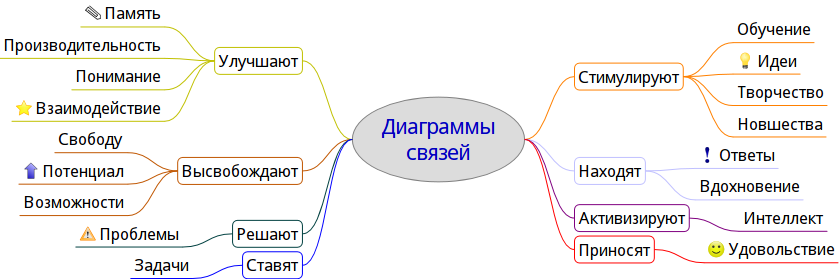
\includegraphics[width=1\linewidth]{mindmap}
  \caption{Пример диаграммы связей}
  \label{pic:mindmap}
\end{figure}

Диаграмма связей состоит из узлов и соединительных линий между ними. Зачастую,
информация, структурированная подобным образом, воспринимается лучше, чем
обычный текст. Оформление диаграммы связей играет большую роль в её восприятии и
осознании. Множество ключевых идей может быть выделено среди всех остальных,
используя атрибуты узла или дуг. К примеру, выделить схожие идеи одинаковым
цветом или поставить пиктограмму напротив некоторых из них. Также существует
возможность скрыть некоторые узлы, чтобы сконцентрироваться на требуемой части
диаграммы. Чем больше доступных способов оформления, тем более точно могут быть
выражены ассоциативные связи между узлами, что в свою очередь способствует
процессу ассоциативного мышления.


\section{Описание проекта HiveMind}
\label{sec:project_summary}
Главной целью проекта HiveMind является разработка редактора диаграмм связей,
удовлетворяющего следующим требованиям: кросс-платформенность, богатая
функциональность, поддержка функций совместного редактирования.

Мобильные устройства получили большое распространение в современном мире.
Зачастую, приложение, предназначенное для на настольного компьютера, неудобно
или невозможно использовать на мобильных устройствах. Специфика мобильных
устройств, по сравнению с настольными компьютерами, заключается в малом
разрешении экрана и наличии альтернативных средств ввода. Данные различия
требуют абсолютно иного подхода к построению пользовательских интерфейсов на
мобильных устройствах. Множество людей пользуются мобильными устройствами вне
дома и настольными компьютерами у себя дома. Пользователь использует множество
операционных систем: Windows, Linux, MacOS на настольных компьютерах и Maemo,
Android, MeeGo на мобильных устройствах. Пользователь нуждается в том, чтобы
необходимое ему приложение было доступно под все виды используемых им платформ.
Данный факт ставит перед разработчиками приложений абсолютно новую задачу  ''---
разработка кросс-платформенных приложений с интерфейсом оптимизированным под
настольные и мобильные платформы \cite{hivemind-8th-fruct}.

Существует множество приложений для редактирования диаграмм связей (FreeMind,
Xmind, Vym, iMindMap и т.д.) и веб-сервисов в сети Интернет (MindMeister,
Mind42, Mindomo и т.д.). Данные редакторы были рассмотрены на предмет
соответствия следующим требованиям:
\begin{itemize}
\item Кросс-платформенность.
\item Широкий функционал.
\item Поддержка функций совместного редактирования.
\item Бесплатность.
\end{itemize}
На текущий момент, не существует редакторов диаграмм связей, удовлетворяющих
вышеперечисленным требованиям \cite{hivemind-8th-fruct}. Поэтому было принято
решение о разработке соответствующего приложения.

В настоящее время, приложение HiveMind обладает следующими возможностями:
\begin{itemize}
\item Чтение и запись файлов в формате FreeMind.
\item Отображение диаграмм связей и навигация по ним.
\item Интерфейс, оптимизированный для настольных и мобильных устройств.
\item Интернационализация.
\item Кросс-платформенность (Поддержка Windows, Linux, Maemo, MeeGo).
\item Использование клавиатуры и сенсорного дисплея.
\end{itemize}


\section{Используемый инструментарий}
\label{sec:toolkit}
Приложение HiveMind написано на языке программирования Python с использованием
библиотеки Qt.

Qt "--- Кросс-платформенный фреймворк, используемый для разработки ПО
~\cite{qt4}. Широко используется для построения приложений с графическим
интерфейсом, так и с интерфейсом командной оболочки. Изначально, библиотека Qt,
написана на C++, но может быть использована на других язык программирования,
используя соответствующие <<привязки>>. Данная библиотека обладает широкой
функциональностью и имеет множество модулей, обеспечивающий работу с 3D
графикой, веб и мультимедиа контентом, базами данных, сетью и т.д.

Python "--- Интерпретируемый, высокоуровневый язык программирования общего
назначения ~\cite{python}. Он нацелен на быстроту написания и легкую читаемость
кода, обладает понятным и минималистичным синтаксисом. Python имеет поддержку
следующих парадигм программирования: объектно-ориентированное, функциональное,
процедурное, аспектно-ориентированное, императивное. Из особенностей языка
следует отметить динамическую типизацию, автоматическое управление памятью,
полную поддержку метапрограммирования и механизм обработки исключений. С данным
языком поставляется большая и многофункциональная библиотека, являющаяся одной
из сильных сторон языка. Помимо всего прочего, язык поддерживает написание
внешних модулей на языках C и C++. Интерпретаторы языка Python доступны под
множеством операционных систем.

PyQt "--- набор <<привязок>> фреймворка Qt для языка программирования Python
~\cite{pyqt4}. PyQt реализует более чем 440 классов и 6000 методов библиотеки
Qt, включающих в себя классы для построения графического интерфейса
пользователя, работы с БД, сетью, XML, SVG и т.д. PyQt лицензирован под двумя
лицензиями: GPL и коммерческой, что позволяет бесплатно использовать его в
проектах с открытым исходным кодом.

Приложение HiveMind является кросс-платформенным и работает под следующими
операционными системами: Windows, Linux, Meego, Maemo. ОС MeeGo ориентирована на
устройства на базе нетбуков, планшетов и ноутбуков, ОС Maemo на мобильные
устройства, в то время как Linux и Windows на настольные компьютеры и ноутбуки.
Каждые из целевых платформ имеют разные форм-факторы, устройства ввода и
соединение с сетью.


\section{Концепция совместного редактирования диаграмм связей}
\label{sec:collaborative_mindmapping}
В общем виде, процесс совместного редактирования диаграмм должен выглядеть
следующим образом. Пользователь, с установленным приложением HiveMind, в любой
момент может открыть доступ к своей диаграмме связей. Другой пользователь
подключается к диаграмме связей данного человека, автоматически получает её
актуальную копию и оба пользователя начинают совместное редактирование
диаграммы. Количество пользователей, участвующих в процессе совместного
редактирования, должно быть неограничено. Пользователь, открывший доступ к
карте, должен иметь возможность изменения прав доступа участников к процессу
совместного взаимодействия. Далее перечисляются возможные сценарии использования
функций совместного редактирования диаграмм связей.

Пользователь создаёт диаграмму связей и начинает её редактирование, используя
мобильное устройство, ноутбук или персональный компьютер. В процессе
редактирования, пользователь решает показать свою работу другу (к примеру, для
получения помощи). Пользователь открывает доступ к своей диаграмме. В данном
случае, устройство, на котором запущено приложение, начинает работать как
сервис, доступный из локальной сети или интернет. Другой пользователь
подключается к диаграмме связей и автоматически получает актуальную копию
диаграммы. Далее оба пользователя начинают совместное редактирование диаграммы.
Количество взаимодействующих участников неограниченно, поэтому другие
пользователи также могут участвовать в совместной работе. Изменения, совершаемые
каждым из участников, незамедлительно посылаются остальным участникам.

Следующий сценарий использования совместного редактирования диаграмм связей
может быть полезен при представлении докладов. К примеру, докладчик имеет
дополнительные материалы, такие как: план презентации, краткий обзор речи
выступления или ссылки на дополнительные ресурсы. Докладчик оформляет данные
материалы в виде диаграммы связей и открывает к ней доступ. Используя HiveMind
на мобильных устройствах или нетбуках, cлушатели подключаются к диаграмме
связей, выложенной докладчиком. Таким образом, слушатели получают материалы
подготовленные докладчиком, а также получают уведомления обо всех изменениях,
сделанных докладчиком в процессе выступуления.

Диаграмма связей может содержать материалы для дискуссии в реальном времени. В
данном случае, она может быть использована, как лекционная доска с иерархической
структурой, на которую каждый участник может заносить свои идеи, комментарии или
мнения. Главное преимущество такого рода обсуждений, с использованием HiveMind,
то, что данные имеют иерархическую структуру и доставляются всем участникам
почти мгновенно.

Пользователь может хранит на диаграмме связей свою личную информацию, поэтому,
открывая доступ к диаграмме, он должен иметь возможность ограничить круг
лиц, имеющих доступ к диаграмме. Также необходимо контролировать права доступа
участников на редактирование диаграммы. К примеру, при выступлении двух
докладчиков перед аудиторией, необходимо разрешить редактирование диаграммы
только выступающим и запретить всем остальным.


\section{Постановка задачи}
\label{sec:problem_statement}
Задача заключается в том, чтобы реализовать возможность совместного
редактирования диаграмм связей в проекте HiveMind.

Существует множество способов установить сетевое взаимодействие между
приложениями, начиная от низкоуровневой обработки пакетов на уровне стека
TCP/IP, заканчивая использованием высокоуровневых объектно-ориентированных
библиотек для протоколов прикладного уровня. С точки зрения реализации,
использование низкоуровневых средств чрезмерно затратно и было решено
использовать высокоуровневую технологию. На сегодняшний день доступно огромное
количество подобных технологий и встаёт задача об её выборе.

Приложение HiveMind нацелено на использование на мобильных и настольных
системах. Значимым различием между двумя типами систем, является их способами
соединения с сетью Интернет, которые отличаются множеством характеристик, такими
как: надёжность, стабильность, ширина полосы пропускания, задержки при передачи
данных и т.д.

Также в составе разных платформ поставляются различные библиотеки и фреймворки.
Из чего следует, что технологии выбираемые для реализации сетевой подсистемы
должны быть доступны под всеми платформами.

Cетевая подсистема должна быть построена на основе существующего приложения.
HiveMind имеет немалую кодовую базу (более 10000 строк кода), большую
функциональность и наличие множества архитектурных решений. Для того чтобы
компенсировать сложность при реализации сетевой подсистемы, она должна быть
выполнена в виде отдельного модуля наименьшим образом связанного с существующими
модулями приложения.



\newpage

\chapter{Реализация}
\label{ch:chapter_2}

\section{Выбор технологий для реализации сетевой архитектуры}

\subsection{Детальная проработка требований}
\label{sec:detailed_requirements}
Существует множество способов установить сетевое взаимодействие между
приложениями, начиная от низкоуровневой обработки пакетов на уровне стека
TCP/IP, заканчивая использованием высокоуровневых объектно-ориентированных
библиотек для протоколов прикладного уровня. Был сформирован ряд ограничений
(см. главу \ref{sec:problem_statement}), которых необходимо придерживаться при
выборе технологии для построения сетевой архитектуры.

В соответствии с концепцией сетевого взаимодействия (см. главу
\ref{sec:collaborative_mindmapping}), мы имеем клиент-серверную архитектуру.
Взаимодействие пользователей будет более удобным, если сервер можно будет
создавать на любом устройстве и в любой момент времени. Взаимодействие должно
выглядеть следующим образом: пользователь создаёт сервер, другие участники
подсоединяются к нему и начинают редактирование. Каждое изменение, сделанное
участником, отправляется на сервер, который рассылает это изменение всем другим
участникам. Для надежного сообщения между клиентами и сервером, все участники
должны иметь одинаковую и верную копию карты.

Проект HiveMind поддерживает мобильные устройства и настольные компьютеры (см.
главу \ref{sec:project_summary}), имеющие различный способ подключения к
интернету. У каждого из этих способов есть свои преимущества и
недостатки. Пользователи настольных компьютеров, как правило, имеют широкий
канал интернет соединения, в отличие от пользователей мобильных устройств.
Мобильные устройства способны подключаться к интернету почти везде и в любое
время. В связи с нехваткой IPv4 адресов, операторы мобильной связи назначают
серые ip адреса мобильным устройствам, что делает данные устройства недоступными
напрямую из сети Интернет. Соединение по беспроводным сетям зачастую нестабильно
и иногда вызывает значительные задержки при передачи данных. Пользователи
настольных компьютеров могут использовать NAT или фаервол блокирующий
входящие соединения. В корпоративной среде, пользователи зачастую ограничены
HTTP прокси, как единственным способом доступа в сеть Интернет.

Подводя итог всем вышеперечисленным особенностям, был сформирован список
требований для выбираемой технологии промежуточного слоя.
\begin{itemize}
\item Взаимодействие основанное на клиент-серверной модели.
\item Сервер должен иметь поддержку подписки.
\item Пользователь может иметь медленное, ненадежное соединение до
сети Интернет, расположенное за NAT.
\item Не должно быть сложностей в создании сервера.
\item Выбранная технология должна поддерживаться библиотекой на языке
Python.
\end{itemize}

\subsection{Преимущества протокола XMPP}
XMPP (Extensible Messaging and Presence Protocol) "--- расширяемый протокол для
обмена сообщениями, в режиме близком к режиму реального времени. Протокол XMPP
может быть рассмотрен на нескольких уровнях абстракции. На нижнем уровне
абстракции, существует клиентское приложение, использующее протокол XMPP,
которое подключается к серверу и обменивается с ним сообщениями. Соединение с
сервером может быть установлено несколькими способами, даже поверх протокола
HTTP. На высоком уровне абстракции, клиент получает доступ ко всей XMPP сети,
где каждый её узел имеет уникальный идентификатор, называемый JID (Jabber
Identificator). Преимуществом является то, что пересылка сообщений между узлами
сети не требует дополнительных усилий. Клиент создаёт сообщение, адресованное
другому клиенту и посылает его на сервер, который отвечает за все операции,
связанные с доставкой данного сообщения.

Большое преимущество протокола XMPP "--- расширяемость. Он может быть расширен
с помощью расширяющих протоколов (XEP). XMPP является открытым протоколом и
каждый желающий может создать высокоуровневый протокол поверх него. Организация
XMPP Standards Foundation отвечает за процесс создания и поддержки данных
протоколов. Существует расширение XEP-0060 Publish-Subscribe \cite{xep-0060}.
Оно отвечает за то, как реализовывать сервис публикации/подписки поверх
протокола XMPP. Любой участник XMPP сети может создать сервис
публикации/подписки.

Протокол XMPP основан на XML, что на первый взгляд может потребовать широкой
полосы Интернет соединения, но это не так. Сообщения между клиентом и сервером
могут быть сжаты с использованием расширения XEP-0138 (Stream Compression
extension).

В настоящее время существует множество общедоступных XMPP серверов
поддерживающих общение в чате. Участие в подобных чатах доступно с мобильных
устройств и не требует широкополосного доступа в Интернет. С технической точки
зрения, совместное редактирование диаграмм очень похоже на участие в чате из
чего следует, что объём трафика не будет сильно отличаться. Исключением является
устройство, являющееся сервером. Данному устройству будет необходим более
широкий канал до сети Интернет для взаимодействия со многими клиентами.

Протокол XMPP c расширением публикации/подписки удовлетворяет требованиям к
технологии промежуточного слоя (см. главу \ref{sec:detailed_requirements}). Он
позволяет избежать почти все сложности связанные с реализацией клиент-серверной
архитектуры и с точки зрения данных требований не имеет недостатков, поэтому он
был выбран технологией промежуточного слоя.


\subsection{Выбор библиотеки для работы с XMPP протоколом}
The next task was to find a pure Python XMPP library that supports XEP-0060
extension. There are eight Python libraries listed at the XMPP Foundation
Website \cite{xmpp}. Some of them are discontinued (jabber.py), some are
targeted at newer (2.6, 3.x) Python releases which are unavailable on Maemo
platform (pyxmpp), the others represent research projects and are not suitable
for production environment (SleekXMPP). Twisted is the only XMPP library
available in Maemo repository.

Twisted framework does not include support for Publish-Subscribe extension but
there is an external full-featured implementation named wokkel.
It is not present in maemo repository. To base our application on top of that 
library, we need to create and maintain package for maemo platform. This is
additional effort we need to make to enable support for mobile devices.

XMPP protocol was created as an instant messaging protocol. It is convenient to
exchange human-readable messages in human-readable format. For the sake of 
interoperability it uses XML-based structures for message formatting. 

\section{Protocol For Collaboration}

% really awful beginning
 The development of any complex protocol and it implementation is a
 labour-consuming process. Our development team had no previous experience in
 such field and thus we decided to use iterative approach. At the first iteration
 protocol for the team work should be as simple as possible. Thereby allow us to
 develop network architecture and to test selected libraries.

 % data structure
 Publish-Subscribe extension requires to share information in the form of nodes
 and items. Node-item system can be compared with file system, where nodes
 represent directories and items represent files. Each item may have unique
 identifier. Subscriber can retrieve items from service either by name or get a
 number of last published items. Items should contain a valid XML data.

 HiveMind has undo/redo capabilities as any good document editor does. Now they
 are implemented on top of QUndoStack. When user makes a change to the mind map
 QUndoCommand is created and pushed into the stack. This allows the user to
 travel through the history of modifications. We decided to use undo/redo stack
 to model data structures of the protocol. All mind map data can be placed
 inside a single node. First item must contain XML-serialized mind map. All other
 items hold small changesets, witch users make to shared map. These modifications
 are the XML-serialized versions of QUndoCommand.

 % notification propagation
 First item in the node is placed by the service in the moment of creation. Other
 items are published by participants of collaboration. Every new modification
 published in the node is retransmitted via update notifications to all
 subscribers and the service holder (see fig. \ref{users_collaboration_example}). 
 Service may reject the changeset if there are some defects (e.g. user wants to 
 update mind map node when it was already deleted by another user) and send error
 notification back to the subscriber.

 Protocol design proposes asynchronous propagation of modifications on the client
 side of publish/subscribe interaction. User changes to the mind map in the form
 of XML-serialized command are transmitted to the service and do not store in
 the local undo stack. Only changesets that were received as update notifications
 are added to the stack.

 Subscribers can retrieve all items stored in the node in any time. This
 way clients may synchronize contents of their local copy of mind map if
 transmitted changeset is rejected. Service does not need any additional effort
 to have up-to-date map because all notifications are local and can not be lost
 during transmission.

 To achieve this asynchronous process new element was added to the core of
 HiveMind --- NetworkController. It manages pub/sub protocol handlers. All
 QUndoCommands created as a result of mind map modifications are passed to the
 controller. If there is no network collaboration at the moment command will be
 sent back to MainWindowController and added to the local undo/redo stack.
 Otherwise command will be serialized and send to the service. Update
 notifications are deserialized into QUndoCommands and added to the undo/redo
 stack.

 The drawbacks of current collaboration protocol design and implementation
 include following statements. Client must wait for an update notification in
 order to see changes that he or she made to the shared mind map. Participants
 cannot use undo/redo commands.

 not 4 current document, may be next one
 There are brilliant examples on how to build iterative update shared space -
 Version Control Systems. Their main aim is almost the same as editing shared
 mind map: provide access to common space of source files. VCS can do all the 
 work here, but they do not provide any notification to all people involved in
 collaborative work. They use robust protocols, send only difference between
 committed versions, and do it really slow. \ldots

\section{Network Subsystem Architecture}

The XMPP protocol family is build out of two things: the core technology and the
XMPP Extension protocols (XEP). The core is responsible for the message exchange
between different parts of the system. Various extension protocols are built on
top of the core. The process of creation and maintenance of such protocols is
managed by XMPP Standards Foundation \cite{xmpp-standarts}.

The XMPP publish-subscribe extension \cite{xep-0060} uses the classic
``publish-subscribe'' or ``observer'' design pattern: a person or application
publishes information, and an event notification (with or without payload) is
broadcasted to all authorized subscribers. In general, the relationship between
the publisher and the subscriber is mediated by a service that receives
publication requests and broadcasts event notifications to subscribers.

Service may support several distinct entities available for subscription. These
entities are called ``nodes''. There are different notification lists for each
node hosted on the service. Publishers send data to the node and subscribers
receive event notifications from it. Nodes can also maintain history of events
and provide other services that supplement the pure pubsub model. Data send to
and from the node is called ``item''.

In terms of publish-subscribe extension the collaboration process can be
described as follows. A user creates a service and a single node for message
exchange. The other participants subscribe to the created node. When anyone
makes a change to the mind map it is sent to the service, which notifies all
participants about the change. The data is sent in the form of the item
payload. Having this principle scheme in mind, we began to form the teamwork
protocol and implement it in detail.

Each change to the mind map is atomic. All changes to the mind map are done with
the use of dialogs. When the edit operation is completed, QUndoCommand is
created and pushed into the command stack. For every change command type XML
serialization and deserialization functions are made.  The use of edit commands
causes the problem of sharing initial contents of the mind map. In order to
execute identical commands, all participants must have exact copies of the
initial mind map. In order to achieve this goal, the first item on the node must
contain XML-serialized mind map. All the other items, as discussed earlier, hold
serialized change commands.  When a participant subscribes to the node he/she
receives all the data stored in the node.

% notification propagation

Each modification published in the node is recorded as a ``changeset''. The
changeset holds information about type of change, time it was formed, and the
author of the change (see fig.~\ref{Changeset propagation}). Service may reject
the changeset if it is irrelevant (e.g. user tries to update mind map node when
it was already deleted by another user) and send error notification back to the
subscriber.

Protocol design proposes asynchronous propagation of modifications on the client
side of publish/subscribe interaction. Modifications to the mind map are
transmitted to the service in the form of XML-serialized commands and are not
stored in the local undo stack. The only changesets received via update
notifications are added to the stack. So, the subscriber must wait for the
correct notification from the service in order to see changes that he or she has
made to the mind map.

The subscribers can retrieve all items stored in the node anytime. This
capability is used to synchronize contents of their local copy of the mind map
if transmitted changeset is rejected. Service does not need any additional
effort to have up-to-date map because all notifications are local and cannot be
lost during transmission.

To implement this asynchronous process, we introduced a new element to HiveMind
core --- NetworkController. It manages publish-subscribe protocol handlers. All
QUndoCommands, created as a result of mind map modifications, are passed to the
controller. If there is no network collaboration at the moment, the command will
be added to the local undo/redo stack. Otherwise, command will be serialized and
sent to the service. Update notifications are deserialized into QUndoCommands
and added to the undo/redo stack.


\section{Implementation of Network Subsystem}

Network subsystem of HiveMind is implemented on top of Twisted \cite{twisted} and
Wokkel \cite{wokkel}. Twisted is a framework for writing asynchronous,
event-driven network applications in Python. It has additional support for many
GUI frameworks like Qt, GTK, Tk, and others.

Wokkel library is a pack of enhancements for Twisted. Particularly, Wokkel
provides a mechanism for easier implementation of XMPP Enhancement Protocols
(XEP). It supports for Service Discovery (XEP-0030), Publish-Subscribe
(XEP-0060) and other XEPs. Implementation of XEP-0060 does not contain business
logic. It means that Wokkel responds for receiving and generating XMPP requests
according to XEP-0060 specification. Wokkel reacts on external pub/sub events
and invokes corresponding methods.

XEP-0060 is very large and complicated. Implementation of all features,
necessary for HiveMind, would take lots of time. Idavoll library is built on top
of Wokkel and provides implementations of many XEP-0060 features such as
``Subscribing'', ``Publishing'', ``Persistent items'', ``Node creation'' and
etc.

Idavoll has many classes needed to implement XEP-0060 specification (see
fig.~\ref{Network classes}). Node class represents a XEP-0060 node. There are
two node types: Leaf and Collection. A leaf node contains a published item,
whereas a collection node contains other nodes.

HivemindNode class inherits LeafNode, but stores the published items in
ChangesetStack instead of a simple list. Using of ChangesetStack allows to check
integrity and correctness of data. Storage class responds for managing all nodes
on the service. BackendService is an implementation of XEP-0060 business logic.
PubSubServiceFromBackend inherits Wokkel's PubSubService class. It invokes
methods for handling corresponding XMPP requests and delegates action performing
to BackendService class.

Mobile devices often have unstable internet connection, so the user have to be
notified when XMPP session is lost. We check connection using XEP-0199 (XMPP
Ping) \cite{ping-xep-0199}. PingClientProtocol class sends ping to the XMPP
server and waits for reply. If there is a certain number of failed pings, the
connection is considered as lost.

The similar mechanism is used for checking participation status of a person. On
the service each participant has his/her own instance of PingClientProtocol. Ping
handler on the client side replies only to the service which it is connected
to. We implemented PingManager class to manage multiple instances of
PingClientProtocol (see fig.~\ref{Ping manager}).  It creates/deletes instances
and starts/stops ping to the certain entity. PingClientProtocol class is
responsible for notifying NetworkController about participant status, which is
shown to the service owner (see fig.~\ref{Permissions dialog}).

\section{Access Control System}
\label{Access control system}

By default, all participants of teamwork have equal permissions to contribute to
the mind map. It is quite convenient for brainstorming-like activities when the
purpose of the collaboration is to generate some materials or to find a solution
for a long-standing problem. This kind of behavior looks unsuitable for other
use cases. Sometimes it is useful to restrict access for particular users in
order to prevent accidental interference of teamwork. To take such scenarios
into account we introduced access control system to HiveMind.

XEP-0060 provides a feature, named Access Model, which can be associated with
authentication system. The user, who creates the mind map, can set trust level
for all new participants i.e. control who can participate in collaboration.
There are four access models implemented in HiveMind:
\begin{itemize}
\item ``Open'' --- any person may join collaboration;
\item ``Roster'' --- only contacts from the owner’s roster may join;
\item ``Authorize'' --- the owner choose who may join on the fly. When a new
  person is connected, the owner gets a participation request from the person;
\item ``Whitelist'' --- a person may join only if he/she is in the owner’s
  whitelist.
\end{itemize}

``Affiliations'' is the next feature, defined in XEP-0060, being a part of
HiveMind access control system. This feature provides authorization capabilities
to XEP-0060. After the person joined collaboration, he/she has a role, which
determines a set of allowed actions. There are four roles implemented in
HiveMind:
\begin{itemize}
\item ``Outcast'' --- person not allowed to join collaboration i.e. in terms of
  IM he/she is banned;
\item ``Member'' --- person allowed to receive items;
\item ``Publisher'' --- person allowed to publish and receive items;
\item ``Owner'' --- similar to the Publisher, but allowed to configure
  collaboration behaviour.
\end{itemize}
Service owner can edit role of desired person at any time with the use of
permissions dialog (fig.~\ref{Permissions dialog}).

XEP-0060 has features that makes access control even more flexible. In some
cases it might be useful to temporarily assign publisher role to all
participants. HiveMind has implementation of XEP-0060 feature named Publish
Model. It determines two cases of who is allowed to make changes to the
mindmap. In the first case it is a person whose affiliation is publisher, and in
the second case any participant is allowed to post changes.

Impelementation of access control system helps us to discover new use cases of
HiveMind. Presentation using HiveMind is one of such use cases. First of all,
lecturer can control who may join the presentation. Secondly, there are can be
more than one lecturer. Presentations using HiveMind distinguish from
collaborative editing: lecturer's current node and fold/unfold events must be
propagated through the network. This ensured that participants can track the
presentation movement.
 
Authorization system can be extended to greatly improve presentation
support. For example, lecturer may want to receive questions. Participants
can add nodes containing a questions or suggestions to lecturer mindmap.
Authorization system controls interaction between lecturer and participants e.g.
participant is able to modify only his own nodes and not able to modify nodes
created by lecturer or other participants.

\chapters{Заключение}

В работе освещена разработка расширений для системы управления проектами
Redmine. Работа была разбита на 3 части.

В первой части были реализованы расширения Redmine, предоставляющие
следующую функциональность:
\begin{itemize}
  \item ораничение доступа к репозиториям;
  \item ограничение доступа к отдельным вики-страницам;
  \item рассылка уведомлений о задачах; 
  \item выбор типа задачи при составлении обзора кода;
  \item механизм позиционирования календаря;
  \item изображения-ссылки в боковой панели.
\end{itemize}

Во второй части был усовершенстован процесс, обеспечивающий поддержку
расширений. Управление данным процессом с помощью инструмента Mercurial Queues,
позволило значительно снизить трудозатраты на поддержку расширений при
обновлениях Redmine.

В третьей части была проведена работа по размещению расширений в открытом
доступе. Благодаря чему, от пользователей были получены отзывы и улучшения,
которые повысили качество расширений.

Разработанные расширения используются в Ярославской лаборатории FRUCT.
Внедрение данных расширений, повысило эффективность и удобство работы
участников лаборатории.



%%% Local Variables: 
%%% mode: latex
%%% TeX-PDF-mode: t
%%% TeX-master: "diploma"
%%% End: 

\addto\captionsrussian{\def\bibname{Список литературы}}
\newpage
\addcontentsline{toc}{chapter}{Литература}
\begin{thebibliography}{99}
%\bibitem{python}
%\textit {Сузи, Р. А.} Язык программирования Python / Р. А. Сузи "---
%Лаборатория знаний, 2007. "--- 328~с.
\bibitem{xep-0060} 
\textit {P. Millard, P. Saint-Andre, R. Meijer.} XEP-0060: Publish-Subscribe
specification. http://xmpp.org/extensions/xep-0060.html

\bibitem{hivemind-8th-fruct}
A. Vasilev, A. Golovchenko, A. Kulikov, I. Paramonov
``HiveMind: Cross-platform Application for Collaborative Mind Mapping,''
\emph{Proceedings of the 8th Conference of Open Innovation Framework
  Program FRUCT}, pp. 219--224, 2010.

\bibitem{xmpp-standarts} The XMPP Standards Foundation http://xmpp.org

\bibitem{xep-0060} P. Millard, P. Saint-Andre, R. Meijer \emph{XEP-0060:
    Publish-Subscribe specification.} http://xmpp.org/extensions/xep-0060.html

\bibitem{twisted} M. Zadka, G. Lefkowitz \emph{The Twisted Network Framework}
  http://twistedmatrix.com/users/glyph/ipc10/paper.html

\bibitem{wokkel} R. Meijer \emph{Wokkel} http://wokkel.ik.nu/

\bibitem{ping-xep-0199} P. Saint-Andre \emph{XEP-0199: XMPP Ping}
http://xmpp.org/extensions/xep-0199.html

\end{thebibliography}
\newpage
\appendix
%\addappheadtotoc
\addcontentsline{toc}{chapter}{Приложение}
\chapter{Скриншоты разрабатываемого приложения}\label{ap:screenshot}

% \begin{figure}[h!] 
% \centering 
% 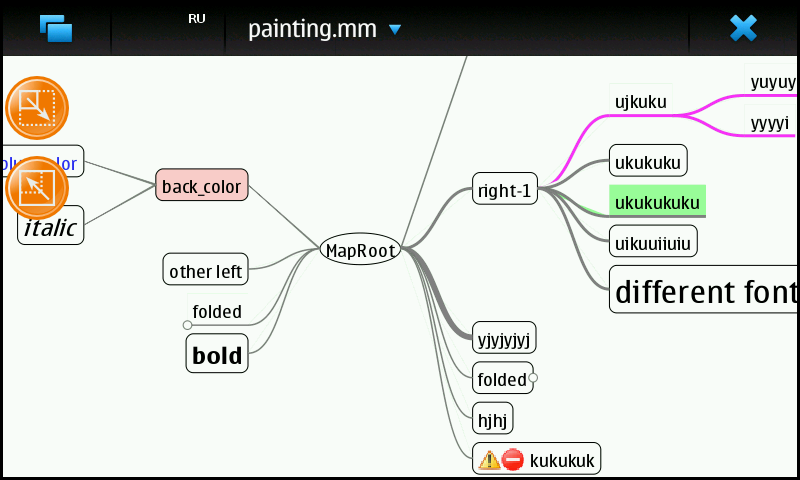
\includegraphics[width=1\linewidth]{main_view} 
% \caption{Отображение модели диаграммы связей}
% \label{ris:main_view}
% \end{figure}
% 
% \begin{figure}[h!] 
% \centering 
% 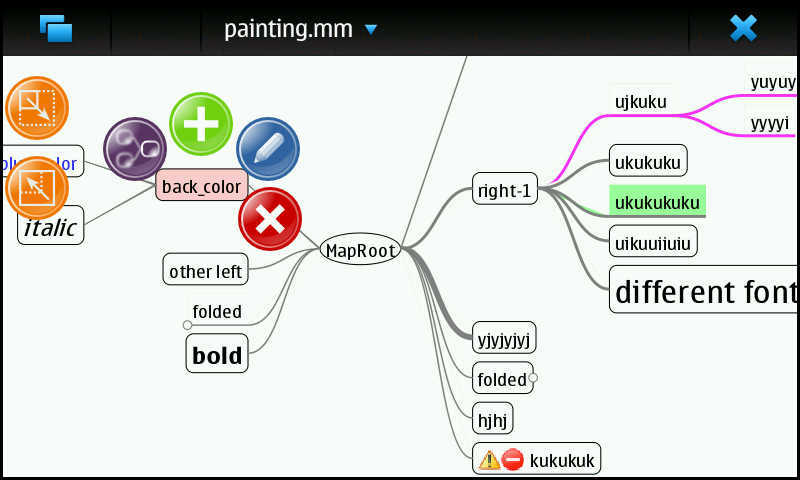
\includegraphics[width=0.6\linewidth]{context_menu} 
% \caption{Контекстное меню узла}
% \label{ris:context_menu}
% \end{figure}
% 
% \begin{figure}[h!]
% \begin{minipage}[h]{0.45\linewidth}
% \center{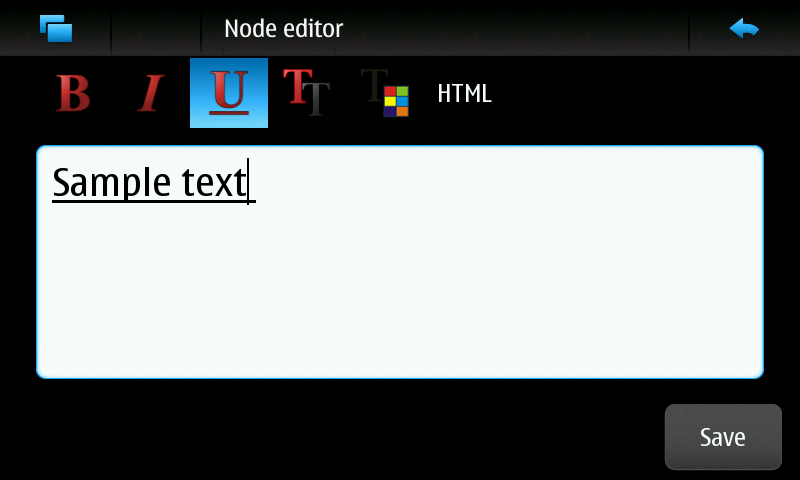
\includegraphics[width=1\linewidth]{text_dialog}} a) Главное окно редактора\\
% \end{minipage}
% \hfill
% \begin{minipage}[h]{0.45\linewidth}
% \center{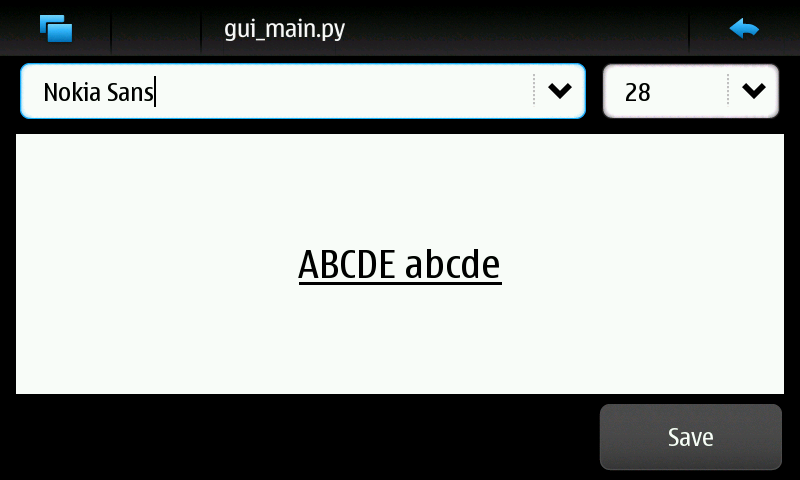
\includegraphics[width=1\linewidth]{font_dialog}} b) Диалог выбора шрифта\\
% \label{ris:font_dialog}
% \end{minipage}
% \vfill
% \begin{minipage}[h]{0.45\linewidth}
% \center{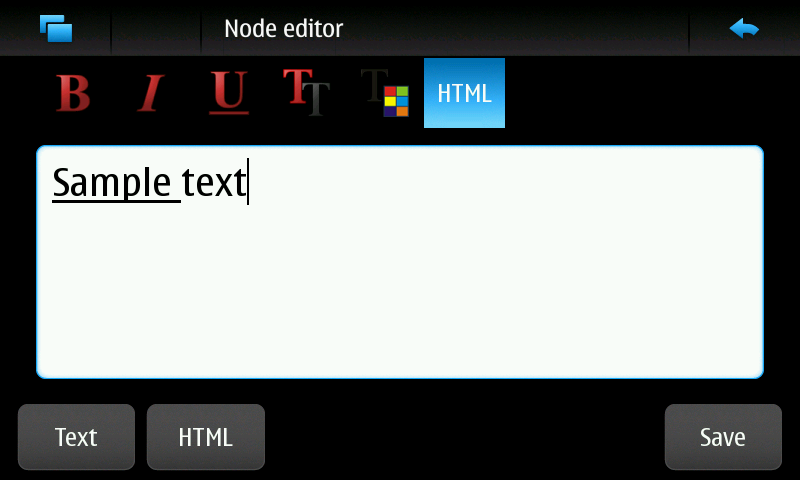
\includegraphics[width=1\linewidth]{html_editor}} c) Режим редактирования HTML\\
% \end{minipage}
% \hfill
% \begin{minipage}[h]{0.45\linewidth}
% \center{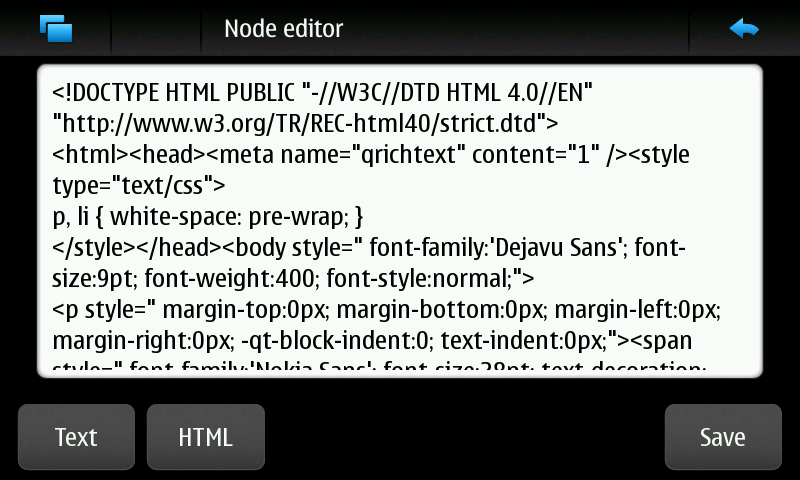
\includegraphics[width=1\linewidth]{html_source}} d) Редактирование исходного кода HTML\\
% \end{minipage}
% \caption{Редактор текста}
% \label{ris:text_editor}
% \end{figure}
% 
% \begin{figure}[h!] 
% \centering 
% 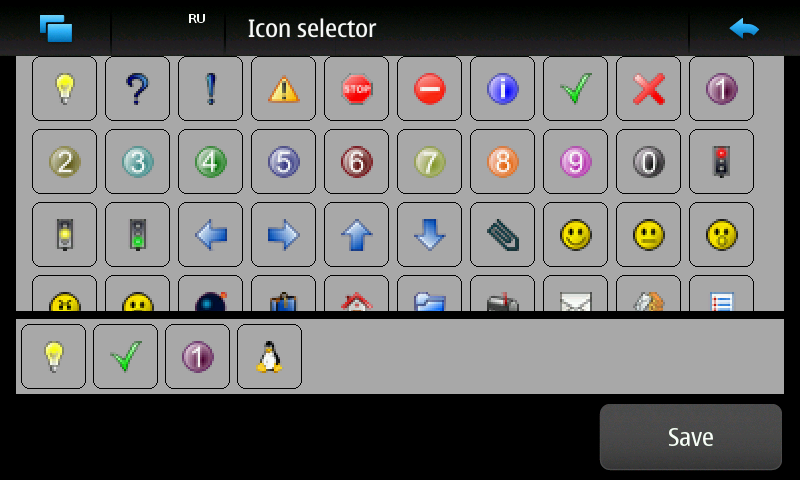
\includegraphics[width=1\linewidth]{icon_selector} 
% \caption{Диалог выбора иконок}
% \label{ris:icons_selector}
% \end{figure}
% \chapter{Диаграмма взаимодействия модели и вида}\label{ap:uml_scene}
% 
% \begin{figure}[h!] 
% \centering 
% 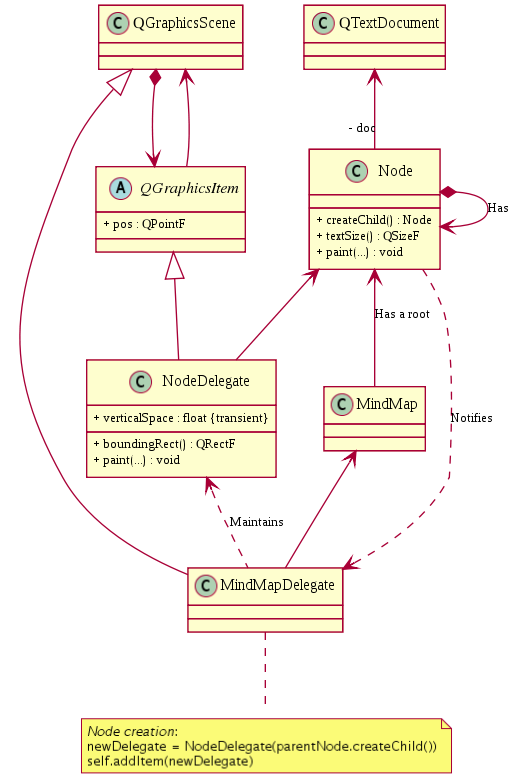
\includegraphics[width=0.5\linewidth]{uml_graphics} 
% \caption{Диаграмма взаимодействия модель-вид}
% \label{ris:uml_scene}
% \end{figure}
\end{document}
